\section{一般映射的扰动分析}
\label{sec:multivariable-differential-perturbation}

输入带有误差时，输出会偏离多少？第~\ref{chap:multivariate-differentiation}章的微分给出一阶预测：输入改变$\bm h$时，输出的变化约为$\mathrm dF_{\bm x}(\bm h)$。把精确变化写成
\[
 \Delta F=F(\bm x+\bm h)-F(\bm x)=\mathrm dF_{\bm x}(\bm h)+R_{\bm x}(\bm h),
\]
本节回答两个问题：在所有允许方向中，一阶误差最多被放大多少倍；对给定的有限步长，一阶预测还差多少。前一个问题由微分的算子范数回答，后一个问题需要控制导数沿扰动线段的变化。

本节的输入、输出空间都是有限维赋范空间，例如取某种范数的$\mathbb R^d$，或按元素排成坐标的矩阵空间。可微性的定义与$\mathbb R^d$中相同；由范数等价（定理~\ref{thm:ls-norm-equivalence}），可微与否不依赖所选范数，只有算子范数的数值依赖范数。

\subsection{局部条件数与导数范数}
\label{sec:multivariable-local-condition-number}

先回顾第~\ref{chap:condition-and-spectral-perturbation}章的结论。对固定矩阵的线性作用$\bm x\mapsto\bm A\bm x$，输出误差与输入误差之比只依赖扰动方向，在全部方向上取上确界，就得到放大倍数$\lVert\bm A\rVert$；相对误差的最坏放大不超过$\kappa(\bm A)=\lVert\bm A\rVert\lVert\bm A^{-1}\rVert$（第~\ref{sec:ls-perturbation-conditioning}节）。这些结论对任意大小的扰动都成立。

一般映射$F$不是线性的，误差比还随扰动大小改变，所以要先在半径为$\delta$的小扰动中取最坏情形，再让半径缩小。

固定基点$\bm x$与输入、输出空间的范数，并设$F$在$\bm x$的一个开邻域内有定义。若只允许对称扰动等结构化变化，就固定一个非零线性子空间$\mathcal E$作为允许的扰动方向，并只在$\bm x+\mathcal E$中取邻域；无结构限制时$\mathcal E$是整个输入空间。
\begin{definition}[局部条件数]
\label{def:multivariable-local-condition-number}
$F$在$\bm x$处相对于允许子空间$\mathcal E$的\term{局部条件数}（local condition number），也称局部绝对条件数，定义为
\begin{equation}
 \kappa_{\mathrm{abs}}(F,\bm x)=\lim_{\delta\downarrow0}\ \sup_{\bm h\in\mathcal E,\ 0<\lVert\bm h\rVert\leq\delta}\frac{\lVert F(\bm x+\bm h)-F(\bm x)\rVert}{\lVert\bm h\rVert}.
\label{eq:multivariable-local-condition-number}
\end{equation}
\end{definition}
内层的上确界覆盖全部允许方向，随$\delta$减小而不增，所以极限在$[0,\infty]$中存在。定义只用到函数值的有限变化，不要求$F$可微。它也不同于沿某个给定方向的响应：后者只是上确界中的一项，最坏方向上的放大可能大得多。

$F$可微时，局部条件数恰好是微分的算子范数。
\begin{theorem}[可微映射的局部条件数]
\label{thm:multivariable-local-condition-number}
若$F$在$\bm x$处可微，则
\begin{equation}
 \kappa_{\mathrm{abs}}(F,\bm x)=\max_{\bm h\in\mathcal E,\ \lVert\bm h\rVert=1}\lVert\mathrm dF_{\bm x}(\bm h)\rVert,
\label{eq:multivariable-local-condition-derivative-norm}
\end{equation}
即微分限制在允许子空间上的算子范数$\lVert\mathrm dF_{\bm x}|_{\mathcal E}\rVert$。
\end{theorem}
\begin{proof}
记余项$R_{\bm x}(\bm h)=F(\bm x+\bm h)-F(\bm x)-\mathrm dF_{\bm x}(\bm h)$，并令
\[
 \eta(\delta)=\sup_{\bm h\in\mathcal E,\ 0<\lVert\bm h\rVert\leq\delta}\frac{\lVert R_{\bm x}(\bm h)\rVert}{\lVert\bm h\rVert}.
\]
可微性说明$\bm h\to\bm0$时$\lVert R_{\bm x}(\bm h)\rVert/\lVert\bm h\rVert\to0$，按极限的定义，$\eta(\delta)\to0$。记$N=\lVert\mathrm dF_{\bm x}|_{\mathcal E}\rVert$。

一方面，由三角不等式，每个比值满足
\[
 \frac{\lVert F(\bm x+\bm h)-F(\bm x)\rVert}{\lVert\bm h\rVert}
 \leq\frac{\lVert\mathrm dF_{\bm x}(\bm h)\rVert}{\lVert\bm h\rVert}+\frac{\lVert R_{\bm x}(\bm h)\rVert}{\lVert\bm h\rVert}
 \leq N+\eta(\delta).
\]

另一方面，有限维线性映射的算子范数可以取到（第~\ref{sec:multivariable-operator-norm}节），取单位向量$\bm h_0\in\mathcal E$使$\lVert\mathrm dF_{\bm x}(\bm h_0)\rVert=N$，令$\bm h=\delta\bm h_0$；由反向三角不等式，
\[
 \frac{\lVert F(\bm x+\bm h)-F(\bm x)\rVert}{\lVert\bm h\rVert}
 \geq\frac{\lVert\mathrm dF_{\bm x}(\bm h)\rVert}{\lVert\bm h\rVert}-\frac{\lVert R_{\bm x}(\bm h)\rVert}{\lVert\bm h\rVert}
 \geq N-\eta(\delta).
\]
所以内层上确界介于$N-\eta(\delta)$与$N+\eta(\delta)$之间，令$\delta\downarrow0$即得。
\end{proof}
所以局部条件数就是最坏方向上的一阶敏感性。若只允许结构化扰动，微分和最坏方向都限制在允许的子空间内，所得数值一般不大于无结构的情形。

\paragraph{相对条件数}
输入、输出的参照量均非零时，把绝对条件数乘以输入尺度、除以输出尺度，得到相对条件数
\[
 \kappa_{\mathrm{rel}}(F,\bm x)=\kappa_{\mathrm{abs}}(F,\bm x)\,\frac{\lVert\bm x\rVert}{\lVert F(\bm x)\rVert},
\]
它衡量相对扰动在一阶上被放大多少倍。

对固定矩阵的线性作用$F(\bm x)=\bm A\bm x$，余项为零，误差比$\lVert\bm A\bm h\rVert/\lVert\bm h\rVert$与步长无关，局部绝对条件数就是$\lVert\bm A\rVert$，相对条件数是$\lVert\bm A\rVert\lVert\bm x\rVert/\lVert\bm A\bm x\rVert$。$\bm A$可逆时，
\[
 \lVert\bm x\rVert=\lVert\bm A^{-1}\bm A\bm x\rVert\leq\lVert\bm A^{-1}\rVert\lVert\bm A\bm x\rVert,
\]
代入后相对条件数不超过$\lVert\bm A\rVert\lVert\bm A^{-1}\rVert=\kappa(\bm A)$，这正回到第~\ref{sec:ls-perturbation-conditioning}节的精确结论。

这里有三个容易混淆的量。矩阵条件数$\kappa(\bm A)$对全部输入取最坏情形，是固定线性作用的统一上界；固定输入$\bm x$处的相对条件数只涉及这一点；把矩阵本身当作输入时，某个矩阵映射（例如求逆）的条件数又是另一个问题，第~\ref{sec:multivariable-matrix-operation-perturbation}节将具体计算。它们描述的都是数学问题本身对输入变化的敏感性；问题条件数与求解算法稳定性的分工见第~\ref{sec:ls-numerical-stability}节，二者不能互相代替。

\paragraph{有限条件数而不可微}
条件数有限并不要求可微。取实对称矩阵$\bm S(t)=\operatorname{diag}(t,-t)$，把$t\in\mathbb R$作为标量输入，输出取排序后的最大特征值$\lambda_{\max}(\bm S(t))=|t|$，两端都用绝对值度量。由Weyl界（定理~\ref{thm:ls-weyl-eigenvalue}），
\[
 |\lambda_{\max}(\bm S(t))-\lambda_{\max}(\bm S(s))|\leq\lVert\bm S(t)-\bm S(s)\rVert_2=|t-s|,
\]
有限变化受到控制；在$t=0$处，比值$|\lambda_{\max}(\bm S(h))-0|/|h|$恒为$1$，所以局部绝对条件数为$1$。

可是$|t|$在$0$处没有双侧导数，这个条件数不能用微分的范数解释。失去可微性的是“排序后取最大”这一步：两条未排序的特征值分支$t$与$-t$本身光滑，它们在$t=0$相交，最大值在交点处从一支换到另一支。第~\ref{sec:multivariable-eigen-differential}节将在特征值简单的条件下，证明所选的局部分支可微。


图~\ref{fig:v2-ordered-eigenvalue-kink}把两条光滑分支与排序后的包络分开画出，可以看见不可微性来自交点处的分支切换。
\begin{figure}[!htb]
\centering
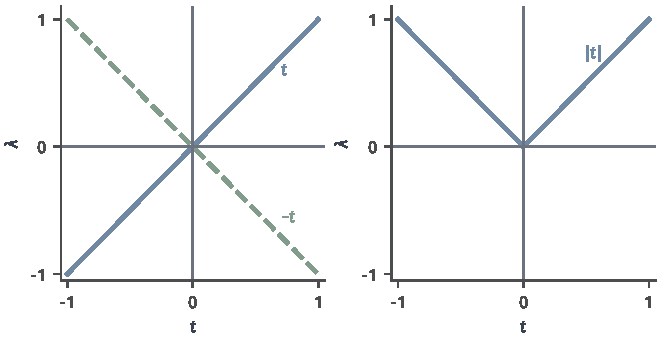
\includegraphics[width=112mm]{figures/02-vectors-matrices-and-multivariate-calculus/04-multivariate-calculus/matplotlib/explanation-additions/ordered-eigenvalue-kink.pdf}
\caption{$\bm S(t)=\operatorname{diag}(t,-t)$。左图为未排序分支$t$与$-t$，右图为最大特征值$|t|$。两侧斜率在零点不同，但函数仍为$1$-Lipschitz，零点的局部绝对条件数仍为$1$。}
\label{fig:v2-ordered-eigenvalue-kink}
\end{figure}

反过来，局部条件数为零也不说明输出不变。$f(t)=t^2$在$0$处导数为零，局部条件数为$0$，但有限步长$t$仍带来变化$t^2$。一阶分析在这里预测“没有变化”，被遗漏的部分要由下一小节的余项界估计。

\subsection{一阶近似的余项界}
\label{sec:multivariable-first-order-remainder}

可微性只保证余项是$o(\lVert\bm h\rVert)$，并不给出某个有限扰动的数值误差界。要得到这样的界，需要知道导数沿扰动线段怎样变化。本小节输入、输出都取欧氏范数，矩阵空间取Frobenius范数，即拉直后的欧氏范数；导数的大小用谱范数度量。其他范数下可借范数等价改变常数。

设$F$在包含线段$[\bm x,\bm x+\bm h]$的开集上连续可微。式~\eqref{eq:multivariable-vector-integral-increment}给出完整增量$\int_0^1\bm J_F(\bm x+t\bm h)\bm h\,\mathrm dt$；从中扣除常向量$\bm J_F(\bm x)\bm h=\int_0^1\bm J_F(\bm x)\bm h\,\mathrm dt$，得到余项的精确表示
\begin{equation}
 R_{\bm x}(\bm h)=F(\bm x+\bm h)-F(\bm x)-\bm J_F(\bm x)\bm h
 =\int_0^1\bigl(\bm J_F(\bm x+t\bm h)-\bm J_F(\bm x)\bigr)\bm h\,\mathrm dt .
\label{eq:multivariable-remainder-integral}
\end{equation}
对照两种估计：完整增量由沿线段的导数大小$\lVert\bm J_F\rVert_2$控制（式~\eqref{eq:analysis-operator-mean-value-bound}），余项则由导数相对基点的变化$\lVert\bm J_F(\bm x+t\bm h)-\bm J_F(\bm x)\rVert_2$控制。导数很大而变化很慢时，整个增量可以很大，一阶预测却仍然准确；二者估计的是不同对象。
\begin{theorem}[一阶近似的二次余项界]
\label{thm:multivariable-first-order-remainder-bound}
设$F$在包含线段$[\bm x,\bm x+\bm h]$的开集上连续可微，且存在常数$L\geq0$，使
\[
 \lVert\bm J_F(\bm y)-\bm J_F(\bm x)\rVert_2\leq L\lVert\bm y-\bm x\rVert_2\qquad(\bm y\in[\bm x,\bm x+\bm h]).
\]
则
\begin{equation}
 \lVert F(\bm x+\bm h)-F(\bm x)-\bm J_F(\bm x)\bm h\rVert_2\leq\frac L2\lVert\bm h\rVert_2^2 .
\label{eq:multivariable-first-order-remainder-bound}
\end{equation}
\end{theorem}
\begin{proof}
取$\bm y=\bm x+t\bm h$，假设给出
\[
 \lVert\bm J_F(\bm x+t\bm h)-\bm J_F(\bm x)\rVert_2\leq Lt\lVert\bm h\rVert_2 .
\]
对式~\eqref{eq:multivariable-remainder-integral}使用向量积分的范数不等式与谱范数的界，
\[
 \lVert R_{\bm x}(\bm h)\rVert_2
 \leq\int_0^1\bigl\lVert\bigl(\bm J_F(\bm x+t\bm h)-\bm J_F(\bm x)\bigr)\bm h\bigr\rVert_2\,\mathrm dt
 \leq\int_0^1Lt\lVert\bm h\rVert_2^2\,\mathrm dt=\frac L2\lVert\bm h\rVert_2^2 .
\]
\end{proof}
定理只要求一阶导数相对基点满足Lipschitz型的界，不以Hessian或二阶导数的存在为前提。若$\bm J_F$在一个凸邻域内以$L$为Lipschitz常数，邻域内每条线段都满足假设。定理~\ref{thm:multivariable-second-derivative-lipschitz}已说明，$F\in C^2$时二阶导数的统一界$M$就是这样的常数，于是余项不超过$M\lVert\bm h\rVert_2^2/2$；这是取得该条件的一种充分办法。

上界正比于$\lVert\bm h\rVert_2^2$：步长缩小到一半，上界缩小到四分之一。这说明的是所保证误差的量级，并不意味着实际误差恰好按同样比例变化，实际误差也可能远小于上界。

例如对称二次型$q(\bm x)=\bm x^\top\bm S\bm x$的Jacobian是$\nabla q^\top=2\bm x^\top\bm S$，满足
\[
 \lVert2\bm S\bm y-2\bm S\bm x\rVert_2\leq2\lVert\bm S\rVert_2\lVert\bm y-\bm x\rVert_2 ;
\]
定理给出余项界$\lVert\bm S\rVert_2\lVert\bm h\rVert_2^2$，与第~\ref{sec:multivariable-differential-rules}节由精确增量得到的$|\bm h^\top\bm S\bm h|\leq\lVert\bm S\rVert_2\lVert\bm h\rVert_2^2$一致。

\paragraph{三种保证的分工}
可微给出统一的$o(\lVert\bm h\rVert)$，只说明步长趋零时的行为；导数的Lipschitz界给出带明确常数的二次余项；第~\ref{sec:multivariable-vector-increment-bound}节的导数界则控制整个有限变化。

使用后两者之前都要先检查：扰动线段是否留在定义域内，可逆、正定等结构条件是否在整条线段上保持，所需常数是否在这个范围内统一成立。矩阵映射的这些检查可以借助已有的有限扰动结论：第~\ref{chap:condition-and-spectral-perturbation}章的Weyl界与奇异值扰动界判断正定性与可逆性是否保持，第~\ref{sec:ls-inverse-sensitivity}节的逆矩阵有限界控制求逆在整段上的变化。基点的条件数只描述无穷小扰动，不能代替这些范围检查和余项估计；下一节对各种矩阵运算逐一完成这些检查。
